%
% slides.tex -- slides
%
% (c) 2017 Prof Dr Andreas Müller, Hochschule Rapperswil
%
\theoremstyle{definition}
\newtheorem{idee}{Idee}
\newtheorem{plan}{Plan}
\newtheorem{kont}{Kontinuitätsgleichung}
\newtheorem{impulserhaltung}{Impulserhaltung}
\newtheorem{ink}{Kompressibilität bewirkt}
\newtheorem{boussinesq}{Boussinesq-Approximation}
\newtheorem{rot}{Rotation}
\newtheorem{sfkt}{Strömungsfunktion}
\newtheorem{divergenz}{Divergenzfreiheit}
\newtheorem{navier}{Navier-Stokes-Gleichung}
\newtheorem{beisp}{Beispiel: Lorenz-Modell}
\newtheorem{anomalie}{Anomalie}

\begin{document}

\ifthenelse{\boolean{presentation}}{
\begin{frame}
\titlepage
\end{frame}
}{}

%
% Warum Fluiddynamik
%
\begin{frame}
\frametitle{Warum Fluiddynamik?}
\begin{idee}
Strömung von Meeren und der Atmosphäre im Detail simulieren und
daraus die zukünftige Entwicklung des Klimas ableiten
\end{idee}
\pause
\begin{plan}
\begin{itemize}[<+->]
\item
Differentialgleichungen für $\varrho$ und $\vec v$ unter der Einwirkung
von Schwerkraft, Coriolis-Kraft und Spannungen (Druck, Viskosität)
aufstellen
\item
Differentialgleichung für Wärme-Transport (Wärmeleitung und -Advektion)
aufstellen
\item
Differentialgleichungen für chemische oder biologishe Prozesse
(auch Änderungen des Aggregatszustandes)
\item
Zustandsgleichungen für $T$, $\varrho$, $\nu$ (Viskosität),
$\kappa$ (Wärmeleitfähigkeit), $c_p$, $c_v$ (Wärmekapazität)
aufstellen
\item
Lösen, fertig \smiley{}
\end{itemize}
\end{plan}

\end{frame}

%
% Warum das nicht geht
%
\begin{frame}
\frametitle{Nicht so schnell \dots}
\begin{itemize}[<+->]
\item
Partielle Differentialgleichungen lösen ist rechenaufwendig,
\item
Mangelnde Genauigkeit für langfristige Rechnung
\item
Viel zu viele Phänomene modelliert, die nichts mit dem Klima zu tun haben
\item
Viel zu hohe Dimensionszahl: Variablen $T$, $p$, $\vec v$, Feuchtigkeit
für jeden Punkt des Raumes und jeden Zeitpunkt
\end{itemize}
\pause
$\Rightarrow$ Nur praktikabel nach dramatischer Vereinfachung
\end{frame}

%
% Modifizierter Plan
%
\begin{frame}
\frametitle{Wie Fluiddynamik?}
\begin{idee}
Strömung von Meeren und der Atmosphäre im Detail simulieren und
daraus die zukünftige Entwicklung des Klimas ableiten
\end{idee}
\pause
\begin{plan}
\begin{itemize}[<+->]
\item
Differentialgleichungen aufstellen%
\uncover<8->{\color{blue}: Kontinuitätsgleichung, Navier-Stokes}
\item
Vereinfachende Annahmen, z.~B.~Inkompressibilität%
\uncover<8->{\color{blue}: Boussinesq-Approximation}
\item
Dimensionsreduktion, z.~B.~Symmetrie%
\uncover<8->{\color{blue}: 2-dimensionale Strömung}
\item
Variablenreduktion%
\uncover<8->{\color{blue}: Strömungsfunktion, Vorticity}
\item
Linearisierung%
\uncover<8->{\color{blue}: abstrakte Klimamodelle}
\item
Entwicklung in endlichdimensionale Basis%
\uncover<8->{\color{blue}: Lorenz-Modell, Zonenmodelle}
\end{itemize}
\end{plan}
\end{frame}

%
% Kontinuitätsgleichung
%
\begin{frame}
\frametitle{Massenerhaltung $\to$ Kontinuitätsgleichung}
Masseänderung in Zeit $\Delta t$  in einem
$\Delta x\times \Delta y\times\Delta z$-Quader
\begin{center}
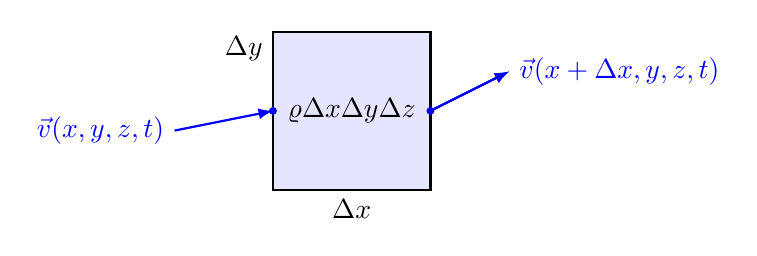
\begin{tikzpicture}[>=latex,thick]
\def\l{1}
\fill[color=blue!10] (-\l,-\l)--(\l,-\l)--(\l,\l)--(-\l,\l)--cycle;
\draw (-\l,-\l)--(\l,-\l)--(\l,\l)--(-\l,\l)--cycle;
\node at (0,-\l) [below] {$\Delta x$};
\node at (-\l, {0.5*\l}) [above left] {$\Delta y$};
\draw[->,color=blue] (\l,0)--({\l + 1},0.5);
\fill[color=blue] (\l,0) circle[radius=0.05cm];
\node[color=blue] at ({\l+1},0.5) [right] {$\vec v(x+\Delta x, y, z, t)$};
\draw[->,color=blue] (\l,0)--({\l + 1},0.5);
\fill[color=blue] (-\l,0) circle[radius=0.05cm];
\draw[<-,color=blue] (-\l,0)--({-\l - 1.25},-0.25);
\node[color=blue] at ({-\l-1.25},-0.25) [left] {$\vec v(x, y, z, t)$};
\node at (0,0) {$\varrho\Delta x\Delta y\Delta z$};
\end{tikzpicture}
\end{center}
\begin{align*}
\onslide<2->{
-\frac{\Delta m}{\Delta t}
&=
(v_x(x+\Delta x,y,z,t)\varrho(x+\Delta x,y,z,t)
-
v_x(x,y,z,t)\varrho(x,y,z,t))
\Delta y\Delta z
+\dots
\\}
\onslide<3->{
-\frac{\Delta\varrho}{\Delta t}
&=
\frac{
v_x(x+\Delta x,y,z,t)\varrho(x+\Delta x,y,z,t)
-
v_x(x,y,z,t)\varrho(x,y,z,t)
}{\Delta x}
+\dots
\\}
\onslide<4->{
-\frac{\partial \varrho}{\partial t}
&=
\frac{\partial(\varrho v_x)}{\partial x}
+
\frac{\partial(\varrho v_y)}{\partial y}
+
\frac{\partial(\varrho v_z)}{\partial z}
=
\nabla\cdot (\varrho\vec v)}
\end{align*}
\end{frame}

%
% Allgemeiner Erhaltungssatz
%
\begin{frame}
\frametitle{Kontinuitätsgleichung $\to$ Erhaltungssatz}
\begin{kont}
\[
-\frac{\partial \varrho}{\partial t}
=
\frac{\partial (\varrho v_x)}{\partial x}+
\frac{\partial (\varrho v_y)}{\partial y}+
\frac{\partial (\varrho v_z)}{\partial z}
\qquad\Leftrightarrow\qquad
\frac{\partial\varrho}{\partial t}=-\nabla\cdot(\varrho\vec v)
\]
\end{kont}
\begin{impulserhaltung}
Impulserhaltung führt auf ``Kontinuitätsgleichung'' Impulsdichte $\varrho\vec v$.
Für jede Komponenten $\varrho v_x$ gilt
\begin{align*}
\onslide<2->{
-\frac{\partial ({\color{red}\varrho v_x})}{\partial t}
&=
\frac{\partial ({\color{red}\varrho v_x}v_x)}{\partial x}
+
\frac{\partial ({\color{red}\varrho v_x}v_y)}{\partial y}
+
\frac{\partial ({\color{red}\varrho v_x}v_y)}{\partial y}
=
\nabla\cdot({\color{red}\varrho v_x}\vec v)
\\}
\onslide<3->{
\frac{\partial (\varrho\vec v)}{\partial t}
&=
-\nabla\cdot(\varrho\vec v\vec v)
\onslide<4->{+\text{Kräfte}}
}
\end{align*}
\end{impulserhaltung}
\end{frame}

%
% Kräfte
%
\begin{frame}
\frametitle{Kräfte}
\begin{navier}
\[
\frac{\partial \varrho\vec v}{\partial t}
=
-\nabla\cdot(\varrho\vec v\vec v)
+\underbrace{\vec g\varrho}_{\displaystyle\text{Schwerkraft}}
-\underbrace{2\varrho\Omega\times\vec v}_{\displaystyle\text{Corioliskraft}}
-\underbrace{\nabla p}_{\displaystyle\text{Druck}}
+\underbrace{\nu \nabla\cdot\sigma\mathstrut}_{\displaystyle\text{Spannungen}}
\]
\end{navier}
\end{frame}

%
% Inkompressibilität
%
\begin{frame}
\frametitle{Inkompressibilität}
\begin{ink}
\begin{itemize}
\item Schallwellen
\item Auftrieb
\end{itemize}
\end{ink}
\begin{boussinesq}
Dichte als Konstant ansehen, ausser beim Auftrieb
\[
\frac{\partial \vec v}{\partial t}
=
-\nabla\cdot(\vec v\vec v)
+\vec g'
-2\Omega\times\vec v
-\frac{1}{\varrho}\nabla p
+\frac{\nu}{\varrho}\nabla\cdot\sigma
\]
Weniger ``schlimm'' nichtlinear.
\end{boussinesq}
\begin{divergenz}
Aus der Kontinuitätsgleichung folgt für $\varrho=\operatorname{const}$
\[
\nabla\cdot\vec v=0
\]
``divergenzfrei''
\end{divergenz}

\end{frame}

%
% Dimensionsreduktion
%
\begin{frame}
\frametitle{2-dimensionale Strömung}
\begin{center}
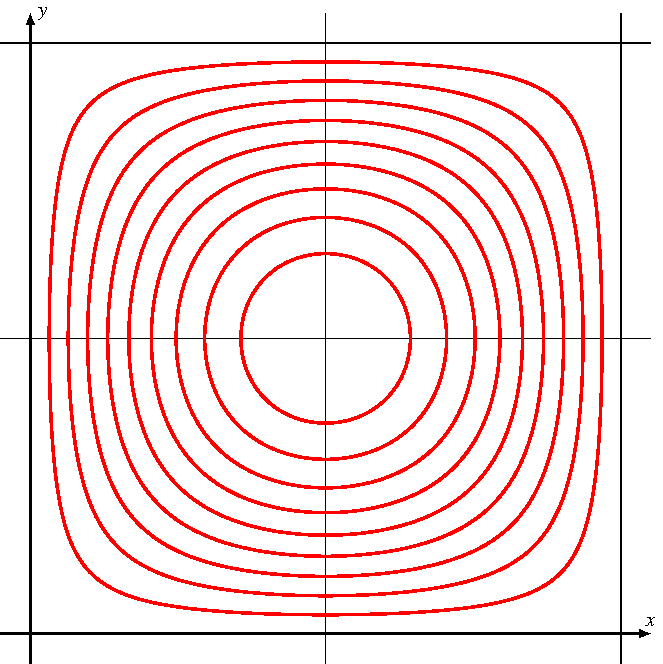
\includegraphics[width=0.5\textwidth]{../../skript/chapters/2/konvektion.pdf}
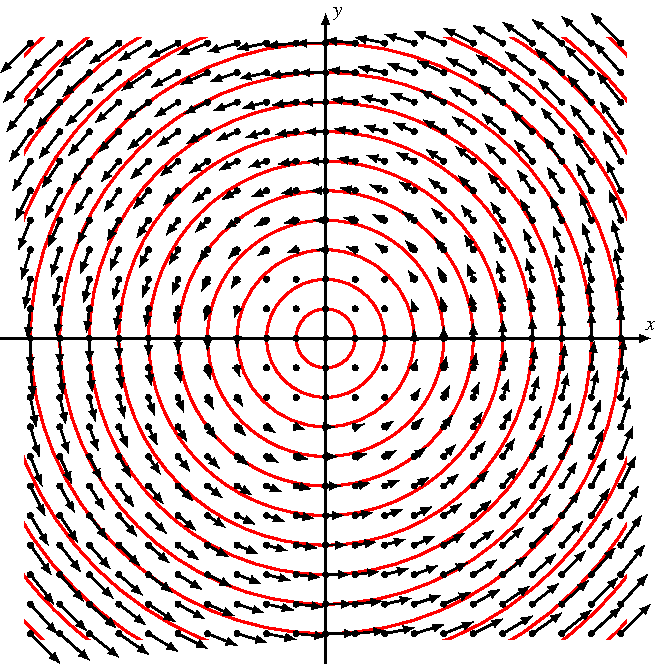
\includegraphics[width=0.5\textwidth]{../../skript/chapters/2/rotation.pdf}
\end{center}
\end{frame}

\begin{frame}
\frametitle{Strömungsfunktion}
\begin{rot}
Gradient um $90^\circ$ drehen:
\[
\vec v
=
\underbrace{\begin{pmatrix}0&-1\\1&0\end{pmatrix}}_{\displaystyle=J}
\nabla (x^2+y^2)
=
J
\begin{pmatrix}
\partial (x^2+y^2)/\partial x\\
\partial (x^2+y^2)/\partial y
\end{pmatrix}
=
J
\begin{pmatrix}
2x\\2y
\end{pmatrix}
=
\begin{pmatrix}-2y\\2x\end{pmatrix}
\]
\end{rot}
\pause
\begin{sfkt}
Wenn $\nabla\cdot\vec v=0$ gilt (inkompressible Strömung), dann kann die
Strömung mit der Stromfunktion $\psi$ beschrieben werden:
\[
\vec v = J \nabla\psi
\]
Reduktion von zwei Funktionen $v_x,v_y$ auf eine: $\psi$.
\end{sfkt}

\end{frame}

%
% Anomalie
%
\begin{frame}
\frametitle{Temperaturprofil}
\begin{columns}
\begin{column}{0.45\textwidth}
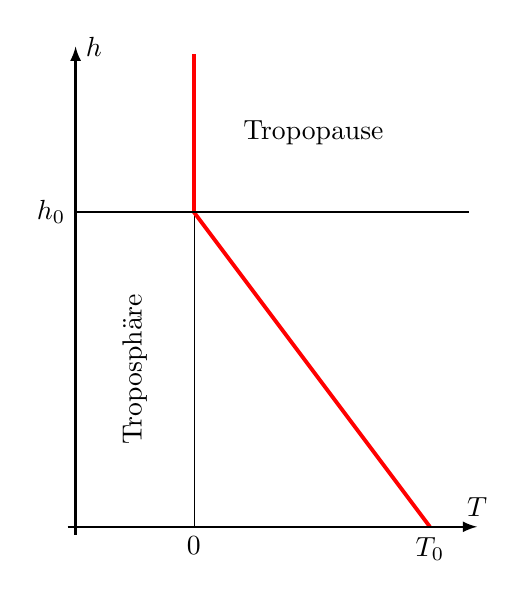
\begin{tikzpicture}[>=latex,thick]
\uncover<2->{
\draw[line width=0.1pt] (1.5,0)--(1.5,4);
}
\draw[line width=1.4pt,color=red] (4.5,0)--(1.5,4);
\draw[line width=1.4pt,color=red] (1.5,4)--(1.5,6);
\draw[line width=0.5pt] (0,4)--(5,4);
\draw[->] (-0.1,0)--(5.1,0) coordinate[label={$T$}];
\draw[->] (0,-0.1)--(0,6.1) coordinate[label={right:$h$}];
\node at (2,5) [right] {Tropopause};
\node at (0.75,2) [rotate=90] {Troposphäre};
\uncover<2->{
\node at (4.5,0) [below] {$T_0$};
\node at (0,4) [left] {$h_0$};
\node at (1.5,0) [below] {$0$};
}
\end{tikzpicture}
\end{column}
\begin{column}{0.52\textwidth}
\uncover<2->{
\begin{beisp}
Temperatur $T=T_0$ für $h=0$ und $T=0$ für $h=h_0$
\begin{align*}
T(h)
&=
T_0\biggl(1-\frac{y}{h_0}\biggr)
\end{align*}
\end{beisp}
}
\uncover<3->{
\begin{anomalie}
Abweichung vom linearen Temperaturprofil:
\[
\vartheta(h)
=
T(h) - 
T_0\biggl(1-\frac{y}{h_0}\biggr)
\]
\end{anomalie}
}
\end{column}
\end{columns}
\end{frame}

\end{document}
